\input{pack.tex}

\title{\LARGE \textbf{MiniRT} - Documentation}
\author{\large Lucie Le Briquer}
\date{\today}

\begin{document}
\maketitle
\tableofcontents
\newpage\rmk On notera dans tout ce document $\scl{\ ,\ }$ le produit scalaire et
$\wedge$ le produit vectoriel.
\section{Génération des rayons}
\begin{center}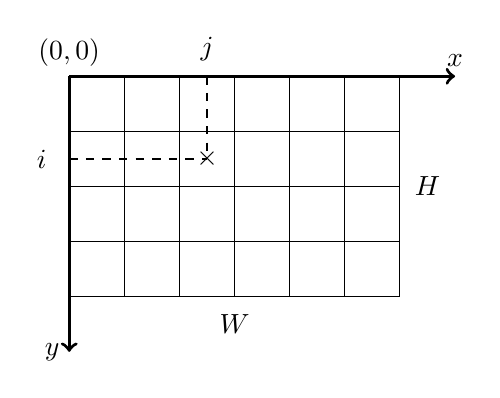
\begin{tikzpicture}[scale=0.7]
	\draw[step=1.0,black,thin] (0,0) grid (6,4);
	\draw[->,very thick] (0,4)--(7,4);
	\draw (7,4) node[above]{$x$};
	\draw[->,very thick] (0,4)--(0,-1);
	\draw (0,-1) node[left]{$y$};
	\draw (0,4) node[left,above]{$(0,0)$};
	\draw (2.5,2.5) node{$\times$};
	\draw (3,-0.5) node{$W$};
	\draw (6.5,2) node{$H$};
	\draw (-0.5,2.5) node{$i$};
	\draw (2.5,4.5) node{$j$};
	\draw[dashed] (0,2.5)--(2.5,2.5);
	\draw[dashed] (2.5,4)--(2.5,2.5);
\end{tikzpicture}
\hspace{1cm}
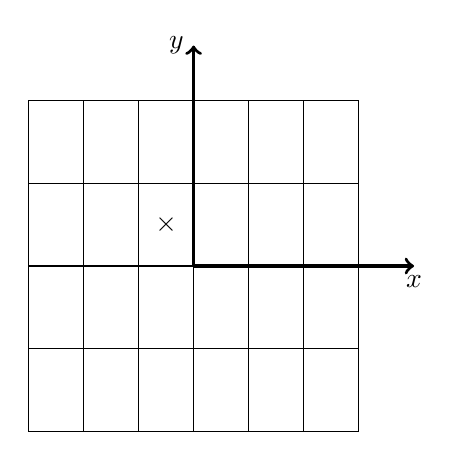
\begin{tikzpicture}[scale=0.7]
	\draw[step=1,yscale=1.5,black,thin] (0,0) grid (6,4);
	\draw[->,very thick] (3,3)--(7,3);
	\draw (7,3) node[below]{$x$};
	\draw[->,very thick] (3,3)--(3,7);
	\draw (3,7) node[left]{$y$};
	\draw (2.5,3.75) node{$\times$};
\end{tikzpicture}\end{center}
\dd\ni On cherche à remplir l'image pixel par pixel, on a $i$ correspondant à la
ligne du pixel et $j$ à sa colonne. On va d'abord normaliser les coordonnées
selon la largeur et la hauteur de l'écran pour travailler avec une image carrée.
On note :
$$\text{pixNorm}_x=\frac{j + 0.5} W \etsp\text{pixNorm}_y\frac{i + 0.5} H$$
\ni On effectue ensuite une translation pour centrer le repère sur le milieu de
l'écran ainsi qu'une inversion de l'axe $y$. Ainsi :
$$\text{pixScreen}_x=2 \times\text{pixNorm}_x -1 \etsp \text{pixScreen}_y = 1 -
2\times \text{pixNorm}_y$$
\ni Il reste ensuite à prendre en compte la FOV donnée en paramètre :
$$\text{pixFinal}_x = \text{pixScreen}_x \times \text{ratio}
\times\tan\left(\frac{\text{FOV}} 2\right)\etsp \text{pixFinal}_y = 
\text{pixScreen}_y \times\tan\left(\frac{\text{FOV}} 2\right)$$
\ni Finalement :
$$\text{pixFinal}_x = \left(2\times \frac{j+0.5}{W}- 1\right)
\times \text{ratio}\times\tan\left(\frac{\text{FOV}} 2\right)$$
$$\text{pixFinal}_y = \left(1 - 2\times \frac{i+0.5}{H}\right)
\times\tan\left(\frac{\text{FOV}} 2\right)$$
\ni où $\text{ratio} = \frac W H$.


\newpage\section{Rotation de la caméra}
\ni Soit $(o_C,\vec{c})$ une caméra, $o_C$ est sa position et $\vec{c}$ la
direction dans laquelle elle regarde. La caméra par défaut regarde en
$(0,0,-1)$.
\begin{center}
\begin{tikzpicture}[scale=0.6]
	\draw[->] (0,0)--(3,0);
	\draw[->] (0,0)--(0,3);
	\draw[->] (0,0)--(-2,-1);
	\draw[->,dashed] (0,0)--(2,1);
	\draw (2.3,1) node[above]{$(0,0,-1)$};
	\draw (0.3,0) node[below]{$0_{\R_3}$};
	\draw (3,0) node[right]{$x$};
	\draw (0,3) node[above]{$y$};
	\draw (-2.3,-1) node[below]{$z$};
	\draw[->] (7,2)--(9.7,2.3);
	\draw[->] (7,2)--(6,0);
	\draw[->] (7,2)--(5.6,4);
	\draw[->,dashed] (7,2)--(8,4);
	\draw (8,4) node[above]{$\vec{c}$};
	\draw (9.7,2.3) node[right]{$X$};
	\draw (5.6,4) node[above]{$Y$};
	\draw (6,0) node[below]{$Z$};
	\draw[dotted] (0,0)--(7,2);
	\draw (0,0) node{$\bullet$};
	\draw (7,2) node{$\bullet$};
	\draw (7.4,2) node[below]{$o_C$};
\end{tikzpicture}
\end{center}
On cherche à déterminer les coordonnées des vecteurs $X,Y$ et $Z$. On sait déjà
que $Z = -\vec{c}$ (normalisé). On cherche maintenant un vecteur $\vec{v}$ tel que :
$$X = v\wedge Z$$
Or on sait que pour $Z = (0,0,1)$ on veut $X = (1,0,0)$. On prend donc $\vec{v}
= (0,1,0)$ pour satisfaire la relation.
$$X = (0,1,0)\wedge Z$$
\rmk Ceci n'est valable que dans le cas ou $Z\neq\lambda (0,1,0)$.
\dl\ni Pour finir la création de la base orthonormée directe on pose donc :
$$Y = Z\wedge X$$
\rmk Pour le cas où $\vec{c} = (0,1,0)$ ou $(0,-1,0)$ on pose $X = (1,0,0)$ (cf
schémas).
\begin{center}
\begin{tikzpicture}[scale=0.6]
	\draw[->] (0,0)--(3,0);
	\draw[->] (0,0)--(0,3);
	\draw[->] (0,0)--(-2,-1);
	\draw (0.3,0) node[below]{$0_{\R_3}$};
	\draw (3,0) node[right]{$x$};
	\draw (0,3) node[above]{$y$};
	\draw (-2.3,-1) node[below]{$z$};
	\draw[->] (7,0)--(10,0);
	\draw[->] (7,0)--(7,3);
	\draw[->] (7,0)--(9,1);
	\draw (10,0) node[right]{$X$};
	\draw (7,3) node[above]{$Z$};
	\draw (9,1) node[right]{$Y$};
	\draw (7,0) node{$\bullet$};
	\draw (0,0) node{$\bullet$};
	\draw[->,dashed] (7,0)--(7,-2.5);
	\draw (7,-2.5) node[below]{$\vec{c}(0,-1,0)$};
	\draw[->] (14,0)--(17,0);
	\draw[->] (14,0)--(14,-3);
	\draw[->] (14,0)--(16,1);
	\draw (17,0) node[right]{$X$};
	\draw (14,-3) node[below]{$Z$};
	\draw (16,1) node[right]{$Y$};
	\draw (14,0) node{$\bullet$};
	\draw[->,dashed] (14,0)--(14,2.5);
	\draw (14,2.5) node[above]{$\vec{c}(0,1,0)$};
\end{tikzpicture}
\end{center}

\newpage\section{Intersection rayon-sphère}
\ni Soit $(o_r, \vec{d}_r)$ le rayon pour lequel on cherche une intersection
avec une sphère ($o_r$ est l'origine du rayon, $\vec{d}_r$ sa direction). Soit $o$ le
centre de la sphère $\Sl$ et $r$ son rayon. On cherche donc un point $p$ de la forme
:
$$p = o_r + \bt \vec{d}_r\quad \bt>0$$
\ni intersectant la sphère, donc vérifiant :
$$\|p - o\|^2 = r$$
\ni On veut donc :
\begin{align*}
	&\|o_r - o + \bt \vec{d}_r\|^2=r^2\\
	\Lra\quad&\bt^2\|\vec{d}_r\|^2 + 2\bt\scl{\vec{d}_r, o_r - o} 
	+\|o_r - o\|^2 =r^2\\
	\Lra\quad&\bt^2 + 2\bt\scl{\vec{d}_r, o_r - o} +\|o_r - o\|^2 =r^2
\end{align*}
\ni Le déterminant est :
$$\Delta = 4\times\left(\scl{\vec{d}_r, o - o_r}^2 - \|o - o_r\|^2 - 
r^2\right)$$
\ni Il ne reste plus qu'à determiner la plus petite racine positive si elle
existe. Si le déterminant est négatif ou que les racines (ou la racine double)
sont négatives, l'intersection n'est pas visible depuis la caméra.

\section{Intersection rayon-plan}
\ni Soit $(o,\vec{n})$ le plan $\Pl$, ou $\vec{n}$ est la normale au plan et $o$
un point du plan. Comme précédemment on cherche un point $p$ de la forme :
$$p = o_r + \bt \vec{d}_r\quad \bt>0$$
\ni intersectant le plan, donc vérifiant :
$$\scl{p - o, \vec{n}} = 0$$
\ni On veut donc :
\begin{align*}
	&\scl{o_r + \bt \vec{d}_r - o + \bt, \vec{n}}=0\\
	\Lra\quad&\scl{o_r - o, \vec{n}} + \bt \scl{\vec{d}_r,\vec{n}}=0\\
\end{align*}
Ainsi :
$$\bt = \frac{\scl{o - o_r, \vec{n}}}{\scl{\vec{d}_r,\vec{n}}}$$
\ni Si $\bt$ est bien positif il y a une intersection visible avec le plan.

\newpage\section{Intersection rayon-triangle}
\ni Soient $(a,b,c)$ les sommets d'un triangle. La première étape est de
vérifier qu'il existe un $\bt$ tel que $p$ soit dans le plan du triangle. On a
donc besoin d'une normale au triangle, on prend par exemple $\vec{n} = (b - a)
\wedge(c - a)$.
\dd\ni On veut maintenant vérifier que le point $p$ est dans le demi-plan
$P_{a,b}$ (où $P_{a,b}$ contient $c$ et est délimité par la droite passant par
$a$ et $b$).
\begin{center}
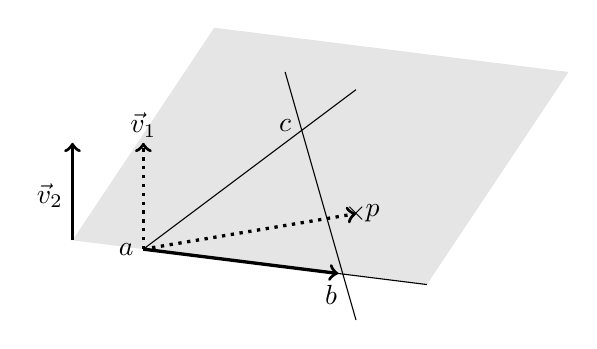
\begin{tikzpicture}[scale=0.45]
	\fill[gray!20] (-2,0.25)--(8,-1)--(12,5)--(2,6.25)--cycle;
	\draw (0,0)--(8,-1);
	\draw (0,0)--(6,4.5);
	\draw[->,very thick] (0,0)--(5.5,-0.6875);
	\draw (0,0) node[left]{$a$};
	\draw (5.3,-1.3) node{$b$};
	\draw (4,3.5) node{$c$};
	\draw (4,5)--(6,-2);
	\draw[->,very thick,dotted] (0,0)--(0,3);
	\draw (0,3.5) node{$\vec{v}_1$};
	\draw[->,very thick] (-2,0.25)--(-2,3);
	\draw (-2,1.5) node[left]{$\vec{v}_2$};
	\draw (6,1) node{$\times$};
	\draw (6,1) node[right]{$p$};
	\draw[->,very thick,dotted] (0,0)--(6,1);
\end{tikzpicture}
\hfill
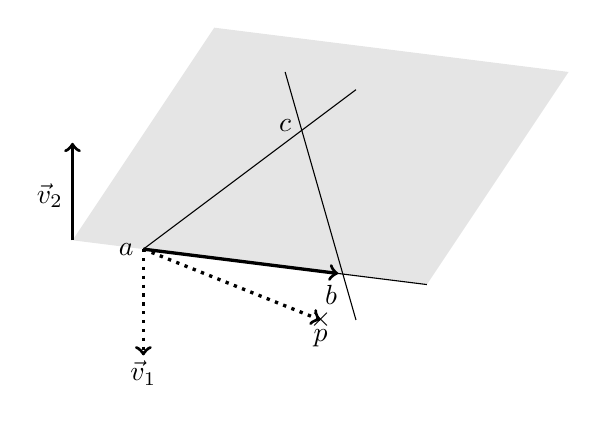
\begin{tikzpicture}[scale=0.45]
	\fill[gray!20] (-2,0.25)--(8,-1)--(12,5)--(2,6.25)--cycle;
	\draw (0,0)--(8,-1);
	\draw (0,0)--(6,4.5);
	\draw[->,very thick] (0,0)--(5.5,-0.6875);
	\draw (0,0) node[left]{$a$};
	\draw (5.3,-1.3) node{$b$};
	\draw (4,3.5) node{$c$};
	\draw (4,5)--(6,-2);
	\draw[->,dotted,very thick] (0,0)--(0,-3);
	\draw (0,-3.5) node{$\vec{v}_1$};
	\draw[->,very thick] (-2,0.25)--(-2,3);
	\draw (-2,1.5) node[left]{$\vec{v}_2$};
	\draw (5,-2) node{$\times$};
	\draw (5,-2) node[below]{$p$};
	\draw[->,very thick,dotted] (0,0)--(5,-2);
\end{tikzpicture}
\end{center}
\dd\ni Il suffit de regarder le signe du produit scalaire entre les deux
vecteurs suivants :
$$\vec{v}_1 = (b - a)\wedge(p - a)\etsp \vec{v}_2 = (b - a)\wedge(c - a)$$
\ni Les deux cas possibles sont representés sur la figure : $\vec{v}_1$ est
orienté comme $\vec{v}_2$ si $p$ est dans le demi-plan, à l'opposé sinon. Ainsi :
$$p\in P_{a,b}\quad\Lra\quad
\scl{(b  a)\wedge(p - a), (b - a)\wedge(c - a)} > 0$$
\ni De même :
$$p\in P_{b,c}\quad\Lra\quad
\scl{(c - b)\wedge(p - b), (c - b)\wedge(a - b)} > 0$$
$$p\in P_{c,a}\quad\Lra\quad
\scl{(a - c)\wedge(p - c), (a - c)\wedge(b - c)} > 0$$
Donc $p$ appartient au triangle ssi :
$$\sys{\scl{(b - a)\wedge(p - a), (b - a)\wedge(c - a)} > 0\\
\scl{(c - b)\wedge(p - b), (c - b)\wedge(a - b)} > 0\\
\scl{(a - c)\wedge(p - c), (a - c)\wedge(b - c)} > 0}$$

\dd\dd\section{Intersection rayon-carré}
\ni Le principe est identique à l'intersection rayon-triangle : on cherche 
d'abord un point qui appartient au plan du carré puis on rajoute
des conditions. Les conditions ici sont : $|y| < \frac h 2$ et $|x|<
\frac h 2$ avec $x$ et $y$ les coordonnées de $p$ dans la base du carré et $h$
la hauteur du carré. On obtient cette base notée $(o,X,Y,Z)$ en suivant les instructions de la
Section 2. On rappelle que :
$$x = \scl{p - o, X} \etsp y = \scl{p - o, Y}$$

\newpage\section{Intersection rayon-cylindre}
\ni Soit $(o,X,Y,Z)$ le repère du cylindre $\Cl$. Le point $p\in\Cl$ ssi
$$x_p^2 + y_p^2 = r^2\etsp|z_p|\leq\frac h 2$$
\ni avec $(x_p,y_p,z_p)$ les coordonnées de $p$ dans le repère du
cylindre. Pour déterminer les vecteurs $(X,Y,Z)$ il suffit d'utiliser la même
construction de base vue précédemment avec comme axe de départ l'axe du cylindre.

\begin{center}
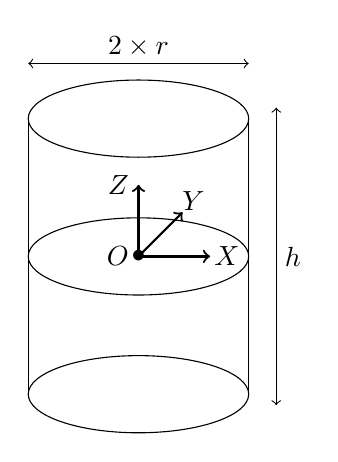
\begin{tikzpicture}[scale=0.7]
	\draw (0,0) ellipse (2cm and 0.7cm);
	\draw (0,2.5) ellipse (2cm and 0.7cm);
	\draw (0,-2.5) ellipse (2cm and 0.7cm);
	\draw (-2,2.5)--(-2,-2.5);
	\draw (2,2.5)--(2,-2.5);
	\draw (0,0) node{$\bullet$};
	\draw (0,0) node[left]{$O$};
	\draw[->,thick] (0,0)--(0,1.3);
	\draw[->,thick] (0,0)--(1.3,0);
	\draw[->,thick] (0,0)--(0.8,0.8);
	\draw (0,1.3) node[left]{$Z$};
	\draw (1.2,0) node[right]{$X$};
	\draw (1,1) node{$Y$};
	\draw[<->] (-2,3.5)--(2,3.5);
	\draw[<->] (2.5,-2.7)--(2.5,2.7);
	\draw (2.8,0) node{$h$};
	\draw (0,3.8) node{$2\times r$};
\end{tikzpicture}
\end{center}
\dd Le point $p$ est de la forme $o_R + \bt d_R$ où $o_R$ est l'origine du rayon et
$d_R$ sa direction. Ainsi :
$$x_p = \lng p - o, X\rng = \bt\scl{d_R, X} + \scl{o_r - o, X}$$
$$y_p = \lng p - o, Y\rng = \bt\scl{d_R, Y} + \scl{o_r - o, Y}$$
Donc,
\begin{align*}
	x_p^2 + y_p^2 = &\left(\scl{d_R,X}^2 + \scl{d_r,Y}^2\right) \bt^2\\
		&+2\left(\scl{d_R,X}\scl{o_R-o,X}+\scl{d_R,Y}\scl{o_R-o,Y}\right) \bt \\
		&+\left(\scl{o_R-o, X}^2 + \scl{o_R-o,Y}^2\right)
\end{align*}
\ni$\bt$ vérifie donc une équation du second degré $a\bt^2+b\bt+c=0$ avec :
$$\sys{a = \scl{d_R,X}^2 + \scl{d_r,Y}^2\\\\
b = 2\left(\scl{d_R,X}\scl{o_R-o,X}+\scl{d_R,Y}\scl{o_R-o,Y}\right) \\\\
c = \scl{o_R-o, X}^2 + \scl{o_R-o,Y}^2 - r^2
}$$
\ni Il reste à vérifier que, pour un des deux $\bt$, on obtient
un point $p$ vérifiant $|z_p|\leq\frac h 2$ sachant que :
$$z_p = \lng p - o, Z\rng = \bt\scl{d_R, Z} + \scl{o_r - o, Z}$$

\end{document}
